\DiaryEntry{Vector Quantization, I}{2021-08-09}{Coding}

We have seen that by grouping source outputs together and encoding them as a single block, we can obtain efficient lossless and lossy compression schemes. So far, we looked at quantization of single samples. Here, we look at ways of quantizing blocks of samples, or vectors. This increases our flexibility and allows us to take dependence between samples into account. Conceptually, we will still be doing the same thing; partitioning the space of inputs into a number of sets, or quantization regions, and then representing each quantization region with a single value. The difference lies in what a region is for scalar values and what it can mean for vector values. In the scalar case, there is only one shape for a quantizer — an interval — and the only question is the size and placement of the interval. In the case of vector-valued samples, there are an infinite number of possible shapes for the interval. This flexibility comes at the cost of increased complexity. Not only do we have to deal with question of the shape of the quantization regions, the number of quantization regions goes up exponentially with the size of the vector.

\subsection{Introduction}

\paragraph{Example.} Suppose we want to quanize the height and weight of individuals; the height of these individuals varies uniformly between $40$ and $80$ inches, and the weight varies uniformly between $40$ and $240$ pounds. Suppose we are allowed a total of $6$ bits to represent each pair of values. We could use $3$ bits to quantize the height and $3$ bits to quantize the weight. Thus, the weight range between $40$ and $240$ pounds would be divided into eight intervals of equal width of 25 and with reconstruction values $\{52, 77, . . . , 227\}$. Similarly, the height range between $40$ and $80$ inches can be divided into eight intervals of width five, with reconstruction levels $\{42, 47, . . . , 77\}$. The following Figure shows the 2-dimensional plot of weight and height.

\begin{figure}[H]
    \centering
    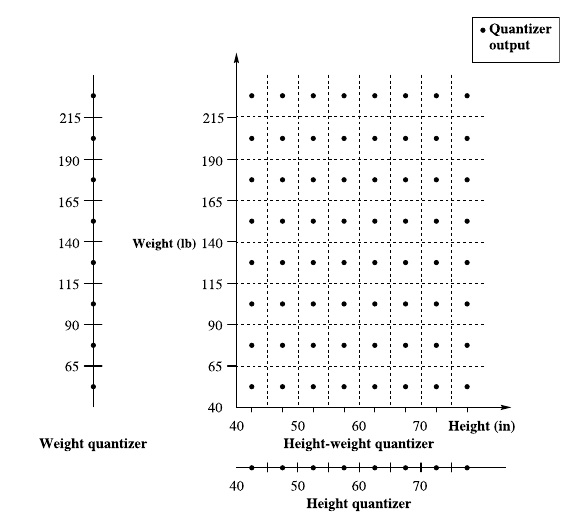
\includegraphics[scale=0.55]{images/2021-08-09_vector_quant_01.png}
\end{figure}

We can see that we effectively have a quantizer output for a person who is $80$ inches tall and weighs $40$ pounds, as well as a quantizer output for an individual whose height is $42$ inches but weighs more than $200$ pounds. Obviously, these outputs will never be used, as is the case for many of the other outputs.

The following Figure shows a "usual" distribution of individuals and we can see a strong correlation between weight and height. We could use a quantizer based on this distribution; this quantizer has exactly the same number of output points as the previous quantizer; however, the output points are clustered in the area occupied by the input. Using this quantizer, we can no longer quantize the height and weight separately. We have to consider them as the coordinates of a point in two dimensions in order to find the closest quantizer output point. However, this method provides a much finer quantization of the input.

\begin{figure}[H]
    \centering
    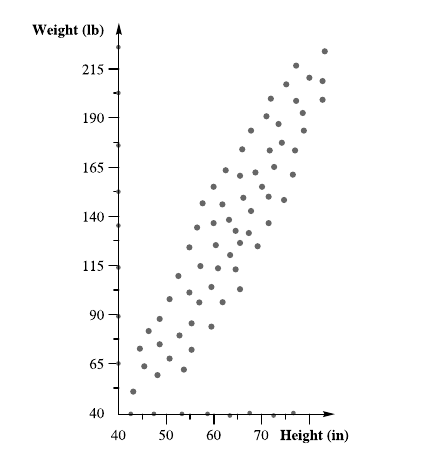
\includegraphics[scale=0.55]{images/2021-08-09_vector_quant_02.png}
\end{figure}

We can see from this example that, as in lossless compression, looking at longer sequences of inputs brings out the structure in the source output. This structure can then be used to provide more efficient representations.

\paragraph{Notation.} We consider vector-valued inputs $\xbf$ which are mapped to quantizer outputs $\ybf_j$ as follows

\bee
Q(\xbf) = \ybf_j \quad \text{if} \,\, d(\xbf, \ybf_j) < d(\xbf, \ybf_i) \, \forall i \neq j
\eee

The quantization regions $V_j$ are then defined as follows

\bee
V_j = \{ \xbf: d(\xbf, \ybf_j) < d(\xbf, \ybf_i) \, \forall i \neq j \}
\eee

Regions defined in this way are often called Voronoi regions. From a multidimensional point of view, using a scalar quantizer for each input restricts the output points to a rectangular grid. Observing several source output values at once allows us to move the output points around. Another way of looking at this is that in one dimension the quantization intervals are restricted to be intervals, and the only parameter that we can manipulate is the size of these intervals.

When we divide the input into vectors of some length $n$ the quantization regions are no longer restricted to be rectangles or squares. We have the freedom to divide the range of the inputs in an infinite number of ways.

\subsection{Design of Vector-based Quantizer}

\paragraph{The Linde-Buzo-Gray algorithm.} When the source distribution is known, the solution to the one-dimensional problem is the Lloyd algorithm. In case of multiple dimensions, this can be extended to the Linde-Buzo-Gray algorithm. This algorithm is not very practical because the integrals required to compute the distortions and centroids are over odd-shaped regions in $n$ dimensions, where $n$ is the dimension of the input vectors. Generally, these integrals are extremely difficult to compute, making this particular algorithm more of an academic interest.

Of more practical interest is the algorithm for the case where we have a training set available. In this case, the algorithm looks very much like the k-means algorithm.

\begin{enumerate}
    \item Start with an initial set of reconstruction values $\{ \ybf_i \}, i=1,\ldots, M$ and training vectors $\{ \xbf_i \}, i=1,\ldots, N$. Set $k=0, D^{(0)} = 0$.
    \item The quantization regions $V_i$ are given by
    
    \bee
        V_i^{(k)} = \{ \xbf_n: d(\xbf_n, \ybf_i) < d(\xbf_n, \ybf_i), \, \forall j \neq i \}, \quad i=1, \ldots, M
    \eee

    \item Calculate the mean distortion $D^{(k)}$
    
    \bee
        D^{(k)} = \frac{1}{N} \sum_i \sum_{\xbf_n \in V_i^{(k)}} || \xbf_n - \ybf_i ||^2
    \eee

    \item If the mean distortion calculated before is "low enough", we stop; other we update the reconstruction values $\ybf_i$ as the average of the elements in each of the quantization regions.

\end{enumerate}

\paragraph{Tree-structured Vector Quantizers.} One way we can introduce structure is to organize our codebook in such a way that it is easy to pick which part contains the desired output vector. Divide the set of output points into two groups, group0 and group1, and assign to each group a test vector such that output points in each group are closer to the test vector assigned to that group than to the test vector assigned to the other group. Label the two test vectors $0$ and $1$. When we get an input vector, we compare it against the test vectors. Depending on the outcome, the input is compared to the output points associated with the test vector closest to the input. After these two comparisons, we can discard half of the output points. If the total number of output points is $K$, with this approach we have to make $K/2 + 2$ comparisons instead of $K$ comparisons.

This process can be continued by splitting the output points in each group into two groups and assigning a test vector to the subgroups. So group0 would be split into group00 and group01, with associated test vectors labeled $00$ and $01$, and group1 would be split into group10 and group11, with associated test vectors labeled $10$ and $11$. Suppose the result of the first set of comparisons was that the output point would be searched for in group1. The input would be compared to the test vectors $10$ and $11$. If the input was closer to the test vector $10$, then the output points in group11 would be discarded, and the input would be compared to the output points in group10. We can continue the procedure by successively dividing each group of output points into two, until finally, if the number of output points is a power of two, the last set of groups would consist of single points. The number of comparisons required to obtain the final output point would be $2 \log K$ instead of $K$. Thus, for a codebook of size $4096$ we would need $24$ vector comparisons instead of $4096$ vector comparisons.



%%% Local Variables:
%%% mode: latex
%%% TeX-master: "journal"
%%% End:
